
\subsection{Webapplikation}\label{Web}
Dieses Kapitel beschäftigt sich mit der Visualisierung der Daten über Plotly Dash. \\
\vspace{3mm}
Um die Daten in der Applikation darzustellen, wurde zuerst eine Verbindung mittels UDP (siehe Kap: \ref{empfang}) erstellt. Somit konnte eine kabellose Verbindung zu einem Laptop hergestellt werden, welcher anschließend alle Sensordaten in einer CSV-Datei einspeichert (siehe Kap. \ref{csv}). Auf dem Laptop wurde Plotly Dash verwendet, um alle Daten darzustellen. Dash eignet sich für solch eine Aufgabe, da über die Python Library einfach dynamische Graphen generiert werden können. \\
\vspace{3mm}
Durch die Möglichkeit, über Dash, Diagramme zu vergrößern und Zeitintervalle leicht einzustellen, können die Daten auch einfacher analysiert werden. \\
\vspace{3mm}
Für die Visualisierung der Daten werden Liniendiagramme verwendet, die die Änderung der Sensorwerte über die Zeit einfach darstellen. Um die Genauigkeit der Datenüberwachung zu verbessern, werden für verschiedene Sensoren auch Vergleichssensoren verwendet, um mögliche Fehler auf dem CubeSat zu erkennen.\\
\vspace{3mm}
\subsubsection{Wie funktioniert Dash }
Dash-Anwendungen\autocite{Dash} bestehen aus verschiedenen HTML-Elementen, wie Bildern, Texten und Tabellen sowie speziellen Dash-Komponenten für interaktive Graphen und andere Visualisierungen. \\
\vspace{3mm}
Auch bietet Dash durch die Verwendung von „Callbacks“ und Funktionen die Möglichkeit interaktive Elemente darzustellen. 

\subsubsection{Callbacks }\label{sec:Callback}
Sogenannte „Callbacks“ sind im Grunde genommen Funktionen, die automatisch ausgeführt werden, um auf bestimmte Aktionen des Benutzers zu reagieren, wie z.B. Klicks auf einen Button, Eingaben in ein Textfeld oder Änderungen in einem Dropdown-Menü.\\
\vspace{3mm}
Die Grundidee hinter den „Callbacks“ in Dash besteht darin, dass sie eine Verbindung zwischen den Eingabeelementen (Input), mit denen der Benutzer interagiert, und den Ausgabeelementen (Output), die aktualisiert werden sollen, herstellen.\\
\vspace{3mm}
Die „Callback-Funktion“ wird jedes Mal aufgerufen, wenn ein Input-Event ausgelöst wird. Diese Funktion führt den Code aus, der notwendig ist, um basierend auf den Eingabewerten neue Ausgabewerte zu berechnen.\\
\vspace{3mm}
Der Dekorator ‚@app.callback‘  wird  in einem Dash Programm verwendet, um ein „Callback“ zu definieren. Anschließend folgt die Definition von Input- und Output-Parameter der Funktion.\\
\vspace{3mm}
\begin{figure}[H]
    \centering
    \begin{minted}{python}
    @app.callback(
		Output('ausgabe', 'children'),  #Ziel
		[Input('texteingabe', 'value')]  #Quelle
		)
    \end{minted}
    \caption{Beispiel eines Callbacks}
\end{figure}
Dash eignet sich am besten bei der Verwendung einer weiteren Python Bibliothek namens „Plotly“. Diese Bibliothek wird für die Darstellung von interaktiven Graphen in Python verwendet und ist auch das Grundgerüst der Dash Bibliothek.

\subsubsection{HTML-Objekte in Dash}
In Dash werden HTML-Objekte durch die Verwendung der ‚dash\_html\_components‘-Bibliothek eingebunden. Somit wird ermöglicht, HTML-Elemente als Python-Objekte zu erstellen und gleich wie in einer HTML-Datei zu manipulieren. \\
\vspace{3mm}
Jedes HTML-Objekt muss Teil des vordefinierten ‚Layouts‘ sein. Ein HTML-Element kann durch „html.“, mit dem Namen des anschließenden Elements erstellt werden. Somit kann ein Titel, welcher in HTML mit dem Tag  ‚<h1>‘  erstellt wird, in Python mit der Codezeile ‚html.H1‘ erstellt werden. \\
\vspace{3mm}
Jede HTML-Komponente in Dash hat eine Reihe von Attributen, die auch den normalen HTML-Attributen entsprechen. Somit werden zum Beispiel für CSS – Klassen die Attribute ‚className‘ verwendet.
\vspace{3mm}
Beispiel für eine HTML-Struktur in einem Python-Dash-Programm: 
\begin{figure}[H]
    \centering
    \begin{minted}{html}
   app.layout = html.Div(children=[
   		 html.H1(children='Test Program’),
   		 html.Div(children='''
       		 Beispiel einer HTML-Struktur in Python 
   		 '''),
	])

    \end{minted}
    \caption{Beispiel HTML-Struktur}
\end{figure}

\subsubsection{Das Programm „dashboard.py“}
Das Programm „dashboard.py“ ist für die Erstellung des interaktiven Web-Dashboards der Teststation zuständig. Das Programm liest die Sensordaten der CSV-Datei ein und stellt sie in Graphen dar. Auch wird das Dashboard periodisch aktualisiert, was für die Anzeige von live aktualisierten Daten nützlich ist.\\
\vspace{3mm}
Zu Beginn werden alle notwendigen Bibliotheken importiert. Darunter die Bibliotheken ‚Dash‘ und ‚plotly.express, da sie für das Web-Dashboard und für die Datenvisualisierung verwendet werden müssen. ‚Flask‘ wird als Webserver verwendet  und ‚pandas‘ ist für die Datenmanipulation und Datenanalyse notwendig. \\
\vspace{3mm}
Zuerst wird der Pfad der CSV-Datei definiert, da sie die empfangenen zu visualisierenden, Daten enthält.

\begin{verbatim}
csv_file_path=' …\\udp_data.csv' #Pfad der CSV-Datei
\end{verbatim}
Anschließend muss der ‚Flask‘-Server und die Dash-App initialisiert werden. Dafür muss eine Instanz für die beiden Objekte erstellt werden. 
\begin{verbatim}
server = Flask(__name__) # Instanz des Flask-Servers
app = dash.Dash(__name__, server=server, suppress_callback_exceptions=True)
#Instanz der Dash App
\end{verbatim}
‘supress\_callback\_exceptions = True’ erlaubt es, Callbacks für nicht sofort verfügbare IDs zu definieren. Dies ist nützlich, da viele Komponenten der Webapplikation dynamisch generiert werden. 
\newpage
\subsubsection{Das HTML-Layout}\label{sec: html layout}
Anschließend wird über das App Layout, die HTML-Struktur der Dash-Applikation gestaltet. \\
\vspace{3mm}
\begin{figure}[H]
    \centering
    \begin{minted}{html}
   dcc.Interval(id='update-interval', interval=5000, n_intervals=0), 
   # Update every 5 seconds
    html.Div([
      html.Div([#Switch for Power Adapter
        html.Div('Power Adapter', className='switch-text'),
        dcc.Checklist(
            id='switch-poweradapter',
            options=[{'label': '', 'value': 'PA'}],
            value=[],
            inputClassName='switch-input',  
            labelClassName='switch-label'
        )
    ], className='switch-wrapper'),
    \end{minted}
    \caption{Beispiel HTML-Layout}
\end{figure}
In dem Codeabschnitt lassen sich zwei verschiedene Arten von Komponenten der HTML-Struktur erkennen. Dash-Core-Komponenten (‚dcc.‘) sind Komponente der HTML-Struktur, welche exklusiv nur mit der Dash-Library verwendbar sind. Alle ‚html.‘-Objekte sind normale HTML-Komponente.\\
\vspace{3mm}
Die regelmäßige Aktualisierung der Benutzeroberfläche wird auch in diesem Layout gesteuert. Durch die Codezeile ‚dcc.Interval()‘ wird die Webseite jede 5s aktualisiert, um hinzugekommene Daten dazustellen.\\
\vspace{3mm}
Über das Objekt ‚dcc.DatePickerRange()‘ kann eingestellt werden in welchem Zeitabschnitt die Daten angezeigt werden sollen.
\begin{figure}[H]
    \centering
    \begin{minted}{html}
   dcc.DatePickerRange(
        id='time-range-selector',
        start_date_placeholder_text="Start Date",
        end_date_placeholder_text="End Date",
        calendar_orientation='horizontal',
    ),
    \end{minted}
    \caption{Beispiel DatePickerRange}
\end{figure}
\vspace{3mm}
Damit nach der Aktualisierung des Programmes nicht das aktuell eingegebene Zeitintervall verloren geht, wird über die ‚.ddc‘-Komponente ‚dcc.store(id = ‚stored-time-range‘)‘ das aktuelle Zeitintervall auf Clientseite, also auf der Seite des Benutzers, gespeichert. \\
\vspace{3mm}
Des Weiteren verfügt das HTML – Layout über verschiedene Schalter, welche zur Steuerung der Aktorik verwendet werden. 
\begin{figure}[H]
    \centering
    \begin{minted}{html}
   html.Div([ #Switch for UV-Lamp
        html.Div('UV-Lamp', className='switch-text'),
        dcc.Checklist(
            id='switch-uvlamp',
            options=[{'label': '', 'value': 'U'}],
            value=[],
            inputClassName='switch-input',
            labelClassName='switch-label'
        )
    ],className='switch-wrapper'), 
    \end{minted}
\end{figure}
Für das Designen der HTML-Oberfläche wird jeder Komponente im Layout eine ‚id‘ (Identifikation) hinzugefügt., da diese Identifikation für die CSS-Datei (Stylesheet) verwendet wird. Auch wird jedem Schalter eine ‚value‘ (Wert) beigefügt. So kann abgefragt werden, ob der Knopf gedrückt wurde oder nicht. 

\subsubsection{Die Funktion ‚generate\_figure‘}
Die Funktion dient zur Generierung der Graphen und beschreibt auch das allgemeine Designthema der Graphen, da für manche ‚.dcc‘-Objekte keine CSS-Stylesheet verwendet werden kann.
\begin{verbatim}
def generate_figure(dataframe, x_column, y_column, title):
\end{verbatim}
\newpage
Die Funktion nimmt insgesamt vier Parameter auf: 
\begin{itemize}
    \item ‚Dataframe‘: Das DataFrame enthält die Daten, die geplottet werden sollen 
    \item x\_column‘: Der Name der Spalte im DataFrame, die auf der X-Achse geplottet werden soll
    \item ‚y\_column‘: Der Name der Spalte bzw. eine Liste von Spaltennamen, die auf der Y-Achse geplottet werden sollen
    \item ‚title‘: Der Titel des Graphen 
\end{itemize}
In der Funktion wird zuerst überprüft, ob ‚y\_column‘ eine Liste ist. Falls dies der Fall ist, ist es möglich, Plots zu erstellen, die mehrere Linien generieren. \\
\vspace{3mm}
\begin{figure}[H]
    \centering
    \begin{minted}{html}
  if isinstance(y_column, list):  
  # Check if multiple y_columns are provided for multiple traces
   fig = px.line(dataframe, x=x_column, y=y_column, title=title)
  else:
   fig = px.line(dataframe, x=x_column, y=y_column, title=title,
   labels={y_column: y_column})
    \end{minted}
\end{figure}
\vspace{3mm}
Falls ‘y\_column’ eine Liste ist, wird ‚px.line‘ mit der X-Spalte und den Y-Spalten als Liste aufgerufen, um mehrere Linien zu plotten.\\
\vspace{3mm}
Wenn ‚y\_column‘ kein Listentyp ist, wird ein einzelner Linienplot erstellt, wobei ‚y\_column‘ als Y-Achsenwert verwendet wird.\\
\vspace{3mm}
Anschließend wird das Layout des Graphen mit der Methode ‚update\_layout‘ aktualisiert. Hierbei werden verschiedene Eigenschaften der Figur angepasst, um ein dunkles Designthema zu erreichen, und um die Lesbarkeit des Graphen zu verbessern. \\
\vspace{3mm}
\begin{figure}[H]
    \centering
    \begin{minted}{python}
  fig.update_layout(
        plot_bgcolor='#002533',  # Dunkler Hintergrund innerhalb
        paper_bgcolor='#00171f',  # Dunkler Hintergrund außerhalb
        font_color='white',  # Weißer Text für bessere Erkennbarkeit
        title_font_color='white',  # Titel Farbe

    \end{minted}
\end{figure}

\subsubsection{Die Callbacks der Website}
Die Callbacks (siehe: Kap.:\ref{sec:Callback}) werden verwendet, um das Dash-Programm mit interaktiven Komponenten zu gestalten. Für das Programm wurden zwei Callback-Funktionen benötigt.\\
\vspace{3mm}
Das erste Callback ist für die Aktualisierung des gespeicherten Zeitbereichs zuständig. Aktualisiert werden dabei die Daten des ‚stored-time-range‘-Objekts, welche auf den vom Benutzer ausgewählten Start- und Enddatumsangaben basieren. 
\vspace{3mm}
\begin{figure}[H]
    \centering
    \begin{minted}{python}
  # Callback um die Graphen, basierend auf die Zeit, zu aktualisieren 
@app.callback(
    Output('stored-time-range', 'data'), #Ausgang gespeichert
    [Input('time-range-selector', 'start_date'), #Eingang: Startdatum
     Input('time-range-selector', 'end_date')], #Ausgang: Enddatum
    prevent_initial_call=True #nicht beim ersten Mal laden
)
    \end{minted}
\end{figure}
‚prevent\_initial\_call = True‘ verhindert, dass das Callback beim ersten Laden der Seite aufgerufen wird, da sonst unnötig Initialisierungen stattfinden können oder ein leerer Aufruf stattfindet. 
Anschließend werden die Start- und Enddaten als Werte in der Funktion ‚update\_stored\_time\_range(start\_date, end\_date)‘ gespeichert. \\
\vspace{3mm}
\begin{figure}[H]
    \centering
    \begin{minted}{python}
    def update_stored_time_range(start_date, end_date):
        return {'start_date': start_date, 'end_date': end_date}

    \end{minted}
\end{figure}
Ziel des zweiten Callbacks ist es, die Eigenschaften des ‚graphs-container‘- Elements zu aktualisieren, was bedeutet, dass alle Graphen basierend auf den aktuellen Daten und Einstellungen neu gerendert werden. 
\vspace{3mm}
\begin{figure}[H]
    \centering
    \begin{minted}{python}
    @app.callback(
     #Ausgang: alle Eigenschaften des 'graphs-container'
    Output('graphs-container', 'children'),
    [Input('update-interval', 'n_intervals')], #Eingang: Timer
    [State('stored-time-range', 'data'), #States der Schalter 
     State('switch-poweradapter', 'value'),
     State('switch-fans', 'value'),
     State('switch-motor', 'value'),
     State('switch-cooler', 'value'),
     State('switch-leds', 'value'),
     State('switch-uvlamp', 'value')]

    \end{minted}
\end{figure}
Der Eingang wird dafür durch den ‚update-interval‘-Timer gesteuert, welcher im Layout (Kap.: \ref{sec: html layout}) definiert wurde. Die verschiedenen Werte der Schalter und des Anfangs- und Enddatums, welche als Zustand im Callback gespeichert wurden, bleiben bei einer Aktualisierung unverändert. 

\subsubsection{Die Funktion ‚update\_args‘}
In der Funktion ‚update\_graphs‘ wird eine Liste von Graphen basierend auf einen gefilterten Datensatz generiert, der durch einen ausgewählten Zeitbereich bestimmt wird. Um dies zu verwirklichen, wird die ‚generate\_figure‘-Funktion in der Funktion verwendet.
\vspace{3mm}
\begin{figure}[H]
    \centering
    \begin{minted}{python}
     #Funktion für die Aktualisierung
    def update_graphs(n_intervals, stored_time_range, *args):
    \end{minted}
\end{figure}
Die Funktion nimmt insgesamt 3 Parameter auf: 
\begin{itemize}
    \item n\_intervals:  Dieser Parameter beschreibt die Anzahl der Intervalle, seit der letzten Aktualisierung.
    \item stored\_time\_range: Ist das oben definierte Dictionary, welches den ausgewählten Zeitbereich abspeichert.
    \item *args: Ist eine Variable, die beschreibt das zusätzliche Argumente in der Funktion benutzt werden können, da die Funktion etwa 8 Parameter einlesen muss aber nur 2 (‚n\_intervals‘ \& ‚stored\_time\_range‘) wirklich benutzt werden. 
\end{itemize}
\vspace{3mm}
In der Funktion wird zuerst überprüft, ob ein Zeitbereich ausgewählt wurde. Falls dies nicht der Fall ist, wird eine leere Liste zurückgegeben, was heißt, dass keine Daten oder Graphen angezeigt werden. Es könnten Callback Fehler vorkommen, falls dies nicht der Fall ist. \\
\vspace{3mm}
Anschließend wird über die Library Pandas die CSV-Datei, welche im oberen Teil des Codes angegeben wurde, ausgelesen. Pandas wird auch für die Umwandlung der Zeit, welche in der CSV-Datei vorhanden ist, in ein DateTime-Format verwendet.\\
\vspace{3mm}
\begin{figure}[H]
    \centering
    \begin{minted}{python}
    df = pd.read_csv(csv_file_path)
    df['Timestamp'] = pd.to_datetime(df['Timestamp'])
    \end{minted}
\end{figure}
Basierend auf dem ausgewählten Zeitbereich wird der DataFrame so gefiltert, dass nur Daten zwischen ‚start\_date‘ und ‚end\_date‘ behalten werden.\\
\vspace{3mm}
\begin{figure}[H]
    \centering
    \begin{minted}{python}
    #Filterung der Daten basierend auf dem ausgewählten Zeitpunkt
    if start_date and end_date:
        filtered_df = df[(df['Timestamp'] >= start_date) & 
        (df['Timestamp']<=             end_date)]
    else:
        filtered_df = df

    \end{minted}
\end{figure}
Nun werden die benötigen Graphen generiert. Für manche Graphen wird dafür auch mehr als nur eine Datenreihe verwendet. 
\vspace{3mm}
\begin{figure}[H]
    \centering
    \begin{minted}{python}
    dcc.Graph(figure=generate_figure(filtered_df, 'Timestamp', 
    ['Gyroscope X', 'Gyroscope Y', 'Gyroscope Z'], 'Gyroscope')),
    \end{minted}
\end{figure}
Die Funktion ‘generate\_figure’, wird benutzt, um aus der entsprechenden Datenreihe eine Figur, bzw. einen Graphen zu erstellen. Dabei werden der gefilterte DataFrame, der Name der ‚Timestamp‘, der Name der Datenspalte und der Titel für den Graphen übergeben.
\subsubsection{Design der Webapplikation }
Die Webapplikation wurde mithilfe von eines CSS-Skript gestaltet und sollte ein dunkles Aussehen haben. Dafür wurden die Farben Schwarz, Weiß, Blau und Grau verwendet. 

\subsubsection{Steuerung von Aktoren}
Um eine Verbindung vom Laptop zum Raspberry PI zu erstellen, um somit alle Aktoren der Teststation zu steuern, muss eine einfache und schnelle Verbindung zwischen den beiden Endgeräten hergestellt werden. 

\subsubsection{MQTT}
Das MQTT-Protokoll\autocite{mqtt} basiert auf einem Publish-Subscribe Modell. In diesem Modell gibt es zwei verschiedene Teilnehmer:
\begin{itemize}
    \item Der MQTT-Client ist eine Anwendung oder ein Gerät, das MQTT-Nachrichten über das Netzwerk (lokal oder global) publiziert (sendet) oder abonniert (empfängt). Sie sind auch für das Erstellen der Verbindung zum Client zuständig.
    \item Ein MQTT-Broker verwaltet die Nachrichtenübertragung zwischen den MQTT-Clients. Der Broker empfängt alle Nachrichten, die von den Clients publiziert werden und filtert diese Nachrichten basierend auf den Themen, zu denen sich andere Clients abonniert haben. Anschließend leitet er diese Nachrichten entsprechend weiter. 
\end{itemize}
Die Korrelation zwischen Client, Broker und Subscriber ist in Abb. 110 veranschaulicht. 
\vspace{3mm}
\begin{figure}[H]
    \centering
    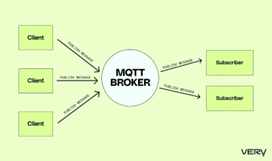
\includegraphics[scale=1]{image/korreation.png}
    \caption{Korrelation\autocite{mqtt-architecture}}
    \label{fig:enter-label}
\end{figure}
\vspace{3mm}
In der Abbildung ist der MQTT-Broker ein reiner Vermittler. Bei der Verbindung zwischen Laptop und Raspberry PI ist jedoch der Einplatinen-Computer sowohl der MQTT-Broker als auch der Subscriber. Der Client ist der Laptop/Computer, welcher Nachrichten über ein bestimmtes Teilgebiet (Topic) veröffentlicht und weiterschickt. Diese Routine dient der Ansteuerung von Aktoren auf dem Raspberry PI, der Benutzer kann den Zustand der verschiedenen Komponenten von dem Laptop aus über ein Dashboard steuern. 

\subsubsection{Fast API}
Schlussendlich wurde anstatt des MQTT-Protokolls die Fast API verwendet (siehe: Kap: \ref{sec:API})\\
\vspace{3mm}
Die Fast API bietet einen leistungsstarken und flexiblen Weg, Aktoren über eine Webanwendung zu steuern. Im Vergleich zu MQTT kann die Nutzung einer API in Bezug auf Netzwerkeffizienz und native Unterstützung von IoT-Geräten eingeschränkt sein. Die API eignet sich für Situationen, in denen komplexe Anfragen zur dynamischen Generierung von Antworten erforderlich sind. MQTT wird hingegen vor allem in Umgebungen eingesetzt, in denen die Effizienz der Nachrichtenübermittlung und der geringe Ressourcenverbrauch im Vordergrund stehen.
